\section*{\nr.2 \tittwo (10 Punkte)}
\begin{enumerate}[(a)]
\item Test
\begin{enumerate}[(1)]
\item Die Kraft, die von einer Ladung auf die Testladung wirkt, wirkt abstoßend und entlang der Verbindungslinie zwischen den beiden
\begin{equation}
  \vec F_i=-a \frac{\vec r_i}{r_i^3}
\end{equation}
mit $a=\frac{2q}{4\pi\epsilon_0}$ und $\vec r_i$ als Ortsvektor der entsprechenden Ladung $i$. Der Einfachheit halber seien im folgenden die Ladungen gegen dem Uhrzeigersinn, beginnend mit der obersten Ladung von $1-5$ numeriert.
Aus Symmetriegründen gleichen sich die $y$-Komponenten der Felder auf der $x$-Achse jeweils paarweise aus, die Felder der beiden Ladungen auf der $y$-Achse gleichen sich im Ursprung deshalb komplett aus, weshalb es genügt die verbleibenden drei Ladungen zu betrachten. 
Die Gesamtkraft auf Ladung 0 ergibt sich dann durch
\begin{equation}
  F_{ges}=F_0\left(1+2\sin\left(\frac{\pi}{4}\right)\right) = F_0\left(1+\sqrt{2}\right),
\end{equation}
wobei die $1$ von Ladung 3 und die $\sin\left(\frac{\pi}{4}\right)$ jeweils von Ladung 2 und 4 kommen.
\item Für die gegebenen Werte ergibt sich 
\begin{equation}
  F_0=5395N \implies F_{ges}=13000N
\end{equation}
\end{enumerate}
\item Für folgende Anordnung ist die Kraft auf die Ladung im Zentrum gleich 0.

\begin{figure}[H]
\centering
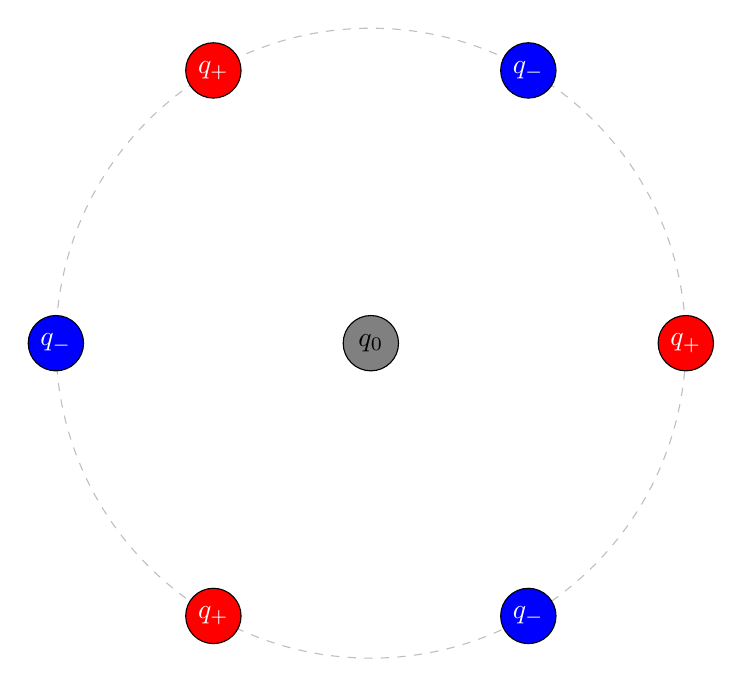
\begin{tikzpicture}

\draw[lightgray, dashed] (0,0) circle (4);
\draw[fill=blue] (-4,0) circle (10pt);
\draw[fill=red] (4,0) circle (10pt);
\draw[fill=blue] (2,3.4641016) circle (10pt);
\draw[fill=red] (-2,3.4641016) circle (10pt);
\draw[fill=red] (-2,-3.4641016) circle (10pt);
\draw[fill=blue] (2,-3.4641016) circle (10pt);
\draw[fill=gray] (0,0) circle (10pt);
\node[white, thick] at (-4,0) {$q_-$};
\node[white, thick] at (4,0) {$q_+$};
\node[white, thick] at (2,3.4641016) {$q_-$};
\node[white, thick] at (2,-3.4641016) {$q_-$};
\node[white, thick] at (-2,-3.4641016) {$q_+$};
\node[white, thick] at (-2,3.4641016) {$q_+$};
\node[black, thick] at (0,0) {$q_0$};

\end{tikzpicture}

\caption{Skizze}
\label{fig:s1}
\end{figure}



\end{enumerate}